\documentclass[11pt]{article}

\newcommand{\yourname}{Kevin Zhang}

\def\comments{0}

%format and packages

%\usepackage{algorithm, algorithmic}
\usepackage{tikz}
\usepackage{algpseudocode}
\usepackage{amsmath, amssymb, amsthm}
\usepackage{tcolorbox}
\usepackage{enumerate}
\usepackage{enumitem}
\usepackage{framed}
\usepackage{verbatim}
\usepackage[margin=1.0in]{geometry}
\usepackage{microtype}
\usepackage{kpfonts}
\usepackage{palatino}
	\DeclareMathAlphabet{\mathtt}{OT1}{cmtt}{m}{n}
	\SetMathAlphabet{\mathtt}{bold}{OT1}{cmtt}{bx}{n}
	\DeclareMathAlphabet{\mathsf}{OT1}{cmss}{m}{n}
	\SetMathAlphabet{\mathsf}{bold}{OT1}{cmss}{bx}{n}
	\renewcommand*\ttdefault{cmtt}
	\renewcommand*\sfdefault{cmss}
	\renewcommand{\baselinestretch}{1.06}

\usepackage[boxruled,vlined,nofillcomment]{algorithm2e}
	\SetKwProg{Fn}{Function}{\string:}{}
	\SetKwFor{While}{While}{}{}
	\SetKwFor{For}{For}{}{}
	\SetKwIF{If}{ElseIf}{Else}{If}{:}{ElseIf}{Else}{:}
	\SetKw{Return}{Return}
	

%enclosure macros
\newcommand{\paren}[1]{\ensuremath{\left( {#1} \right)}}
\newcommand{\bracket}[1]{\ensuremath{\left\{ {#1} \right\}}}
\renewcommand{\sb}[1]{\ensuremath{\left[ {#1} \right\]}}
\newcommand{\ab}[1]{\ensuremath{\left\langle {#1} \right\rangle}}

%probability macros
\newcommand{\ex}[2]{{\ifx&#1& \mathbb{E} \else \underset{#1}{\mathbb{E}} \fi \left[#2\right]}}
\newcommand{\pr}[2]{{\ifx&#1& \mathbb{P} \else \underset{#1}{\mathbb{P}} \fi \left[#2\right]}}
\newcommand{\var}[2]{{\ifx&#1& \mathrm{Var} \else \underset{#1}{\mathrm{Var}} \fi \left[#2\right]}}

%useful CS macros
\newcommand{\poly}{\mathrm{poly}}
\newcommand{\polylog}{\mathrm{polylog}}
\newcommand{\zo}{\{0,1\}}
\newcommand{\pmo}{\{\pm1\}}
\newcommand{\getsr}{\gets_{\mbox{\tiny R}}}
\newcommand{\card}[1]{\left| #1 \right|}
\newcommand{\set}[1]{\left\{#1\right\}}
\newcommand{\negl}{\mathrm{negl}}
\newcommand{\eps}{\varepsilon}
\DeclareMathOperator*{\argmin}{arg\,min}
\DeclareMathOperator*{\argmax}{arg\,max}
\newcommand{\eqand}{\qquad \textrm{and} \qquad}
\newcommand{\ind}[1]{\mathbb{I}\{#1\}}
\newcommand{\sslash}{\ensuremath{\mathbin{/\mkern-3mu/}}}

%mathbb
\newcommand{\N}{\mathbb{N}}
\newcommand{\R}{\mathbb{R}}
\newcommand{\Z}{\mathbb{Z}}
%mathcal
\newcommand{\cA}{\mathcal{A}}
\newcommand{\cB}{\mathcal{B}}
\newcommand{\cC}{\mathcal{C}}
\newcommand{\cD}{\mathcal{D}}
\newcommand{\cE}{\mathcal{E}}
\newcommand{\cF}{\mathcal{F}}
\newcommand{\cL}{\mathcal{L}}
\newcommand{\cM}{\mathcal{M}}
\newcommand{\cO}{\mathcal{O}}
\newcommand{\cP}{\mathcal{P}}
\newcommand{\cQ}{\mathcal{Q}}
\newcommand{\cR}{\mathcal{R}}
\newcommand{\cS}{\mathcal{S}}
\newcommand{\cU}{\mathcal{U}}
\newcommand{\cV}{\mathcal{V}}
\newcommand{\cW}{\mathcal{W}}
\newcommand{\cX}{\mathcal{X}}
\newcommand{\cY}{\mathcal{Y}}
\newcommand{\cZ}{\mathcal{Z}}

%theorem macros
\newtheorem{thm}{Theorem}
\newtheorem{lem}[thm]{Lemma}
\newtheorem{fact}[thm]{Fact}
\newtheorem{clm}[thm]{Claim}
\newtheorem{rem}[thm]{Remark}
\newtheorem{coro}[thm]{Corollary}
\newtheorem{prop}[thm]{Proposition}
\newtheorem{conj}[thm]{Conjecture}

\theoremstyle{definition}
\newtheorem{defn}[thm]{Definition}
\newtheoremstyle{case}{}{}{}{}{}{:}{ }{}
\theoremstyle{case}
\newtheorem{case}{Case}

\theoremstyle{theorem}
\newtheorem{prob}{Problem}
\newtheorem{sol}{Solution}

\tikzset{every picture/.style={line width=0.75pt}} %set default line width to 0.75pt        

\begin{document}
{\large
\noindent Name: \yourname}

\vspace{15pt}

\begin{prob}\end{prob}

\begin{enumerate}[label=(\alph*)]

\item



\tikzset{every picture/.style={line width=0.75pt}} %set default line width to 0.75pt        

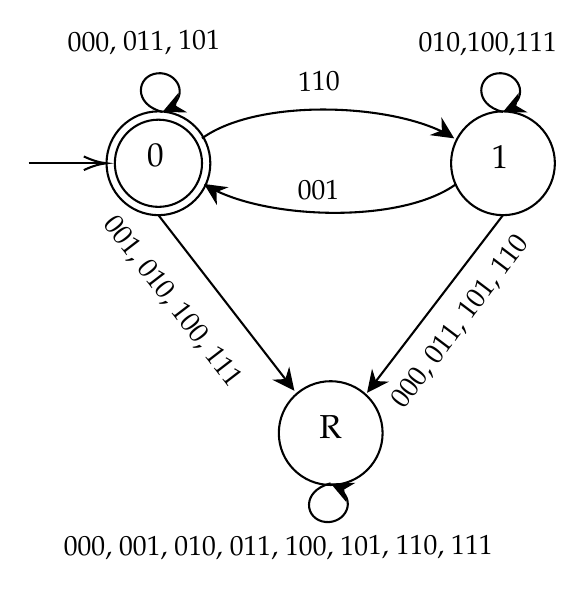
\begin{tikzpicture}[x=0.75pt,y=0.75pt,yscale=-1,xscale=1]
%uncomment if require: \path (0,295); %set diagram left start at 0, and has height of 295

%Shape: Circle [id:dp5003833209957831] 
\draw   (55,80) .. controls (55,66.19) and (66.19,55) .. (80,55) .. controls (93.81,55) and (105,66.19) .. (105,80) .. controls (105,93.81) and (93.81,105) .. (80,105) .. controls (66.19,105) and (55,93.81) .. (55,80) -- cycle ;
%Shape: Circle [id:dp672443205500185] 
\draw   (221,80) .. controls (221,66.19) and (232.19,55) .. (246,55) .. controls (259.81,55) and (271,66.19) .. (271,80) .. controls (271,93.81) and (259.81,105) .. (246,105) .. controls (232.19,105) and (221,93.81) .. (221,80) -- cycle ;
%Straight Lines [id:da6387762500578644] 
\draw    (17.5,80) -- (53,80) ;
\draw [shift={(55,80)}, rotate = 180] [color={rgb, 255:red, 0; green, 0; blue, 0 }  ][line width=0.75]    (10.93,-3.29) .. controls (6.95,-1.4) and (3.31,-0.3) .. (0,0) .. controls (3.31,0.3) and (6.95,1.4) .. (10.93,3.29)   ;
%Curve Lines [id:da2980191576941209] 
\draw    (81.98,55.26) .. controls (67.48,51.66) and (69.48,37.66) .. (79.48,36.66) .. controls (88.83,35.73) and (95.56,47.03) .. (84.54,53.9) ;
\draw [shift={(81.98,55.26)}, rotate = 335.53] [fill={rgb, 255:red, 0; green, 0; blue, 0 }  ][line width=0.08]  [draw opacity=0] (10.72,-5.15) -- (0,0) -- (10.72,5.15) -- (7.12,0) -- cycle    ;
%Curve Lines [id:da6022536579324818] 
\draw    (245.98,55.26) .. controls (231.48,51.66) and (233.48,37.66) .. (243.48,36.66) .. controls (252.83,35.73) and (259.56,47.03) .. (248.54,53.9) ;
\draw [shift={(245.98,55.26)}, rotate = 335.53] [fill={rgb, 255:red, 0; green, 0; blue, 0 }  ][line width=0.08]  [draw opacity=0] (10.72,-5.15) -- (0,0) -- (10.72,5.15) -- (7.12,0) -- cycle    ;
%Curve Lines [id:da6141300036570287] 
\draw    (101,68) .. controls (127.68,48.6) and (192.46,50.84) .. (220.05,66.51) ;
\draw [shift={(222.5,68)}, rotate = 213.18] [fill={rgb, 255:red, 0; green, 0; blue, 0 }  ][line width=0.08]  [draw opacity=0] (10.72,-5.15) -- (0,0) -- (10.72,5.15) -- (7.12,0) -- cycle    ;
%Shape: Circle [id:dp8435127556394624] 
\draw   (59,80) .. controls (59,68.4) and (68.4,59) .. (80,59) .. controls (91.6,59) and (101,68.4) .. (101,80) .. controls (101,91.6) and (91.6,101) .. (80,101) .. controls (68.4,101) and (59,91.6) .. (59,80) -- cycle ;
%Curve Lines [id:da11079201223500545] 
\draw    (223.5,89.98) .. controls (196.83,109.38) and (132.04,107.14) .. (104.45,91.48) ;
\draw [shift={(102,89.98)}, rotate = 393.18] [fill={rgb, 255:red, 0; green, 0; blue, 0 }  ][line width=0.08]  [draw opacity=0] (10.72,-5.15) -- (0,0) -- (10.72,5.15) -- (7.12,0) -- cycle    ;
%Shape: Circle [id:dp9593311748213864] 
\draw   (138,210) .. controls (138,196.19) and (149.19,185) .. (163,185) .. controls (176.81,185) and (188,196.19) .. (188,210) .. controls (188,223.81) and (176.81,235) .. (163,235) .. controls (149.19,235) and (138,223.81) .. (138,210) -- cycle ;
%Straight Lines [id:da2931900074181599] 
\draw    (80,105) -- (143.66,187.23) ;
\draw [shift={(145.5,189.6)}, rotate = 232.25] [fill={rgb, 255:red, 0; green, 0; blue, 0 }  ][line width=0.08]  [draw opacity=0] (10.72,-5.15) -- (0,0) -- (10.72,5.15) -- (7.12,0) -- cycle    ;
%Straight Lines [id:da13474819048557873] 
\draw    (246,105) -- (182.32,188.22) ;
\draw [shift={(180.5,190.6)}, rotate = 307.42] [fill={rgb, 255:red, 0; green, 0; blue, 0 }  ][line width=0.08]  [draw opacity=0] (10.72,-5.15) -- (0,0) -- (10.72,5.15) -- (7.12,0) -- cycle    ;
%Curve Lines [id:da8524028602831142] 
\draw    (162.98,234.22) .. controls (148.48,237.82) and (150.48,251.82) .. (160.48,252.82) .. controls (169.83,253.76) and (176.56,242.45) .. (165.54,235.59) ;
\draw [shift={(162.98,234.22)}, rotate = 384.47] [fill={rgb, 255:red, 0; green, 0; blue, 0 }  ][line width=0.08]  [draw opacity=0] (10.72,-5.15) -- (0,0) -- (10.72,5.15) -- (7.12,0) -- cycle    ;

% Text Node
\draw (73,69) node [anchor=north west][inner sep=0.75pt]  [font=\large] [align=left] {0};
% Text Node
\draw (239,70) node [anchor=north west][inner sep=0.75pt]  [font=\large] [align=left] {1};
% Text Node
\draw (34.74,15.44) node [anchor=north west][inner sep=0.75pt]  [rotate=-359.04] [align=left] {000, 011, 101};
% Text Node
\draw (203.9,15.22) node [anchor=north west][inner sep=0.75pt]  [rotate=-0.15] [align=left] {010,100,111};
% Text Node
\draw (145.74,34.44) node [anchor=north west][inner sep=0.75pt]  [rotate=-359.04] [align=left] {110};
% Text Node
\draw (145.56,86.86) node [anchor=north west][inner sep=0.75pt]  [rotate=-359.6] [align=left] {001};
% Text Node
\draw (156,200) node [anchor=north west][inner sep=0.75pt]  [font=\large] [align=left] {R};
% Text Node
\draw (188.65,193.16) node [anchor=north west][inner sep=0.75pt]  [rotate=-307.16] [align=left] {000, 011, 101, 110};
% Text Node
\draw (32.86,258.26) node [anchor=north west][inner sep=0.75pt]  [rotate=-359.87] [align=left] {000, 001, 010, 011, 100, 101, 110, 111};
% Text Node
\draw (60.79,101.58) node [anchor=north west][inner sep=0.75pt]  [rotate=-52.4] [align=left] {001, 010, 100, 111};


\end{tikzpicture}

$A^R$ must be regular because it is accepted by the automaton above.

\item
$A$ must be regular language, because $A^R$ is a regular language. 
Since $A = (A^R)^R$, and the reversal operation is a regular operation,
$A$ must be a regular language.

\item




\tikzset{every picture/.style={line width=0.75pt}} %set default line width to 0.75pt        

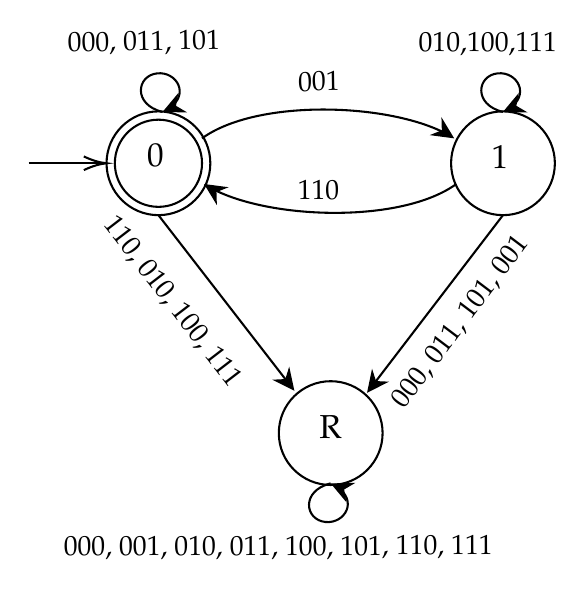
\begin{tikzpicture}[x=0.75pt,y=0.75pt,yscale=-1,xscale=1]
%uncomment if require: \path (0,300); %set diagram left start at 0, and has height of 300

%Shape: Circle [id:dp39467023106716037] 
\draw   (54,79.73) .. controls (54,65.93) and (65.19,54.73) .. (79,54.73) .. controls (92.81,54.73) and (104,65.93) .. (104,79.73) .. controls (104,93.54) and (92.81,104.73) .. (79,104.73) .. controls (65.19,104.73) and (54,93.54) .. (54,79.73) -- cycle ;
%Shape: Circle [id:dp7365821230320577] 
\draw   (220,79.73) .. controls (220,65.93) and (231.19,54.73) .. (245,54.73) .. controls (258.81,54.73) and (270,65.93) .. (270,79.73) .. controls (270,93.54) and (258.81,104.73) .. (245,104.73) .. controls (231.19,104.73) and (220,93.54) .. (220,79.73) -- cycle ;
%Straight Lines [id:da13288390432262354] 
\draw    (16.5,79.73) -- (52,79.73) ;
\draw [shift={(54,79.73)}, rotate = 180] [color={rgb, 255:red, 0; green, 0; blue, 0 }  ][line width=0.75]    (10.93,-3.29) .. controls (6.95,-1.4) and (3.31,-0.3) .. (0,0) .. controls (3.31,0.3) and (6.95,1.4) .. (10.93,3.29)   ;
%Curve Lines [id:da36453721102958747] 
\draw    (80.98,55) .. controls (66.48,51.4) and (68.48,37.4) .. (78.48,36.4) .. controls (87.83,35.46) and (94.56,46.77) .. (83.54,53.64) ;
\draw [shift={(80.98,55)}, rotate = 335.53] [fill={rgb, 255:red, 0; green, 0; blue, 0 }  ][line width=0.08]  [draw opacity=0] (10.72,-5.15) -- (0,0) -- (10.72,5.15) -- (7.12,0) -- cycle    ;
%Curve Lines [id:da21916678887928676] 
\draw    (244.98,55) .. controls (230.48,51.4) and (232.48,37.4) .. (242.48,36.4) .. controls (251.83,35.46) and (258.56,46.77) .. (247.54,53.64) ;
\draw [shift={(244.98,55)}, rotate = 335.53] [fill={rgb, 255:red, 0; green, 0; blue, 0 }  ][line width=0.08]  [draw opacity=0] (10.72,-5.15) -- (0,0) -- (10.72,5.15) -- (7.12,0) -- cycle    ;
%Curve Lines [id:da26608146789072773] 
\draw    (100,67.73) .. controls (126.68,48.33) and (191.46,50.58) .. (219.05,66.24) ;
\draw [shift={(221.5,67.73)}, rotate = 213.18] [fill={rgb, 255:red, 0; green, 0; blue, 0 }  ][line width=0.08]  [draw opacity=0] (10.72,-5.15) -- (0,0) -- (10.72,5.15) -- (7.12,0) -- cycle    ;
%Shape: Circle [id:dp1581309235148214] 
\draw   (58,79.73) .. controls (58,68.14) and (67.4,58.73) .. (79,58.73) .. controls (90.6,58.73) and (100,68.14) .. (100,79.73) .. controls (100,91.33) and (90.6,100.73) .. (79,100.73) .. controls (67.4,100.73) and (58,91.33) .. (58,79.73) -- cycle ;
%Curve Lines [id:da8932916562923463] 
\draw    (222.5,89.72) .. controls (195.83,109.12) and (131.04,106.88) .. (103.45,91.21) ;
\draw [shift={(101,89.72)}, rotate = 393.18] [fill={rgb, 255:red, 0; green, 0; blue, 0 }  ][line width=0.08]  [draw opacity=0] (10.72,-5.15) -- (0,0) -- (10.72,5.15) -- (7.12,0) -- cycle    ;
%Shape: Circle [id:dp5178923943339659] 
\draw   (137,209.73) .. controls (137,195.93) and (148.19,184.73) .. (162,184.73) .. controls (175.81,184.73) and (187,195.93) .. (187,209.73) .. controls (187,223.54) and (175.81,234.73) .. (162,234.73) .. controls (148.19,234.73) and (137,223.54) .. (137,209.73) -- cycle ;
%Straight Lines [id:da7957452142429624] 
\draw    (79,104.73) -- (142.66,186.96) ;
\draw [shift={(144.5,189.33)}, rotate = 232.25] [fill={rgb, 255:red, 0; green, 0; blue, 0 }  ][line width=0.08]  [draw opacity=0] (10.72,-5.15) -- (0,0) -- (10.72,5.15) -- (7.12,0) -- cycle    ;
%Straight Lines [id:da352017054909995] 
\draw    (245,104.73) -- (181.32,187.95) ;
\draw [shift={(179.5,190.33)}, rotate = 307.42] [fill={rgb, 255:red, 0; green, 0; blue, 0 }  ][line width=0.08]  [draw opacity=0] (10.72,-5.15) -- (0,0) -- (10.72,5.15) -- (7.12,0) -- cycle    ;
%Curve Lines [id:da271121958620427] 
\draw    (161.98,233.96) .. controls (147.48,237.56) and (149.48,251.56) .. (159.48,252.56) .. controls (168.83,253.49) and (175.56,242.19) .. (164.54,235.32) ;
\draw [shift={(161.98,233.96)}, rotate = 384.47] [fill={rgb, 255:red, 0; green, 0; blue, 0 }  ][line width=0.08]  [draw opacity=0] (10.72,-5.15) -- (0,0) -- (10.72,5.15) -- (7.12,0) -- cycle    ;

% Text Node
\draw (72,68.73) node [anchor=north west][inner sep=0.75pt]  [font=\large] [align=left] {0};
% Text Node
\draw (238,69.73) node [anchor=north west][inner sep=0.75pt]  [font=\large] [align=left] {1};
% Text Node
\draw (33.74,15.17) node [anchor=north west][inner sep=0.75pt]  [rotate=-359.04] [align=left] {000, 011, 101};
% Text Node
\draw (202.9,14.96) node [anchor=north west][inner sep=0.75pt]  [rotate=-0.15] [align=left] {010,100,111};
% Text Node
\draw (144.74,34.17) node [anchor=north west][inner sep=0.75pt]  [rotate=-359.04] [align=left] {001};
% Text Node
\draw (144.56,86.59) node [anchor=north west][inner sep=0.75pt]  [rotate=-359.6] [align=left] {110};
% Text Node
\draw (155,199.73) node [anchor=north west][inner sep=0.75pt]  [font=\large] [align=left] {R};
% Text Node
\draw (187.65,192.89) node [anchor=north west][inner sep=0.75pt]  [rotate=-307.16] [align=left] {000, 011, 101, 001};
% Text Node
\draw (31.86,258) node [anchor=north west][inner sep=0.75pt]  [rotate=-359.87] [align=left] {000, 001, 010, 011, 100, 101, 110, 111};
% Text Node
\draw (59.79,101.31) node [anchor=north west][inner sep=0.75pt]  [rotate=-52.4] [align=left] {110, 010, 100, 111};


\end{tikzpicture}

\end{enumerate}

\newpage

\begin{prob}\end{prob}

\begin{enumerate}[label=(\alph*)]

\item
$baa \in a^*b^*a^*b^*$ is True, because the $^*$ operator is for zero or more of an element. 
$a^*b^*a^*b^*$ might look like $b^*a^*$, to which fits $baa$.

\item
$a^* \cup b^* = (a \cup b)^*$ is False, because the right hand side (inside parenthesis) is equivalent to $\{a, b\}$.
This, combined with the star operator, means any string with any combination of $a$s or $b$s will work.
In contrast, the left hand side accepts only either strings with only $a$s, or strings with only $b$s, and the empty string.
$aba$ will be accepted by the right, but not by the left.

\item
$(a^*b^*)^* = (a \cup b)^*$ is True. The left side can form any string with any combination of $a$s or $b$s.
This is possible, because the inside of the parenthesis expands out to be $\{\varepsilon, a, b, ab, b, ...\}$,
which has $\{\varepsilon, a, b\}$ as a subset.

\item
$b^*a^* \cap a^*b^* = a^* \cup b^*$ is True, because the only intersection the left side can have is
the same letter repeated. $baaaa$ cannot be in $b^*a^* \cap a^*b^*$, because there is no way to construct it
using $a^*b^*$. Similar argument can be made about $aaaaab$. Therefore, the only elements in such an
interesection are either $a^*$ or $b^*$, the union of which is $a^* \cup b^*$.

\item
$(ab)^*a = a(ba)^*$ is True. Both sequences form a palindrome-like chain of $aba$. The left side looks
like $\{a, aba, ababa, abababa, ... \}$, and the right side forms the same sequence. 

\item
$a^*b^* \cap c^*d^* = \varnothing$ is False. $\varepsilon$ is in both sets, so the intersection should be 
$\{\varepsilon\}$.

\item
$abcd \in (a (cd)^* b)^*$ is False. The right side has $(cd)^*$ between $a$ and $b$, and in $abcd$, $cd$ is after $ab$. 
   
\end{enumerate}

\begin{prob}\end{prob}

\begin{enumerate}[label=(\alph*)]

\item
$(b^*(\varepsilon \cup a \cup ab^*a \cup ab^*ab^*a)b^*)$

\item
$\varepsilon \cup ((a \cup b)^*a) \cup ((a \cup b)^*bb) $

\item
$(b^*ab^*ab^*ab^*)^*$

\end{enumerate}

\newpage

\begin{prob}\end{prob}

\begin{enumerate}[label=(\alph*)]

\item
$(a \cup b)^*$ because that represents any length string of $a$s and $b$s. $(a \cup \varepsilon)b^*$ is not
a strong restriction, because both parts can be $\varepsilon$, and any $a$ or $b$s can then get folded into
$(a \cup b)^*$.

\item
$(a \cup b)^*$ because all the other elements are subsets of $(a \cup b)^*$.

\item
$a^*b$ because if we start looking at the accepted elements, they are $\{b, ab, aab, ...\}$.

\item
$(a \cup b)^*$ because the left side is all elements that end in $b$ (plus $\varepsilon$), 
and the right side is all elements that end in $a$ (plus $\varepsilon$). Since all substrings of $\{a, b\}$ 
end in $a$ or $b$, or is $\varepsilon$, $(a \cup b)^*$ is my answer.

\item
$(a \cup b)^* a (a \cup b)^*$ because the expression cannot be simplified further. The expression
is all strings that have at least one $a$ in it, and there is no other way to indicate all 
possible strings of $\{a, b\}$ BEFORE and AFTER.  

\end{enumerate}

\begin{prob}\end{prob}

\tikzset{every picture/.style={line width=0.75pt}} %set default line width to 0.75pt        

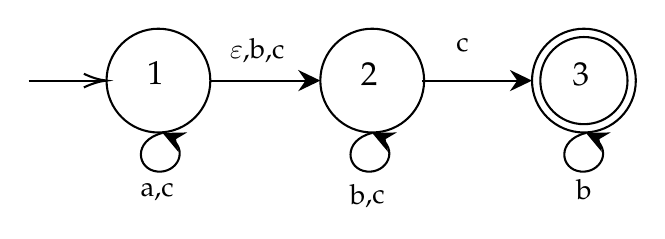
\begin{tikzpicture}[x=0.75pt,y=0.75pt,yscale=-1,xscale=1]
%uncomment if require: \path (0,114); %set diagram left start at 0, and has height of 114

%Shape: Circle [id:dp8389123271259622] 
\draw   (55,39) .. controls (55,25.19) and (66.19,14) .. (80,14) .. controls (93.81,14) and (105,25.19) .. (105,39) .. controls (105,52.81) and (93.81,64) .. (80,64) .. controls (66.19,64) and (55,52.81) .. (55,39) -- cycle ;
%Shape: Circle [id:dp8146907162622614] 
\draw   (158,39) .. controls (158,25.19) and (169.19,14) .. (183,14) .. controls (196.81,14) and (208,25.19) .. (208,39) .. controls (208,52.81) and (196.81,64) .. (183,64) .. controls (169.19,64) and (158,52.81) .. (158,39) -- cycle ;
%Straight Lines [id:da8369906022529925] 
\draw    (17.5,39) -- (53,39) ;
\draw [shift={(55,39)}, rotate = 180] [color={rgb, 255:red, 0; green, 0; blue, 0 }  ][line width=0.75]    (10.93,-3.29) .. controls (6.95,-1.4) and (3.31,-0.3) .. (0,0) .. controls (3.31,0.3) and (6.95,1.4) .. (10.93,3.29)   ;
%Straight Lines [id:da978352783596667] 
\draw    (105,39) -- (155,39) ;
\draw [shift={(158,39)}, rotate = 180] [fill={rgb, 255:red, 0; green, 0; blue, 0 }  ][line width=0.08]  [draw opacity=0] (10.72,-5.15) -- (0,0) -- (10.72,5.15) -- (7.12,0) -- cycle    ;
%Curve Lines [id:da7147206862906095] 
\draw    (81.98,64.22) .. controls (67.48,67.82) and (69.48,81.82) .. (79.48,82.82) .. controls (88.83,83.76) and (95.56,72.45) .. (84.54,65.59) ;
\draw [shift={(81.98,64.22)}, rotate = 384.47] [fill={rgb, 255:red, 0; green, 0; blue, 0 }  ][line width=0.08]  [draw opacity=0] (10.72,-5.15) -- (0,0) -- (10.72,5.15) -- (7.12,0) -- cycle    ;
%Shape: Circle [id:dp34647223802509175] 
\draw   (264,39) .. controls (264,27.4) and (273.4,18) .. (285,18) .. controls (296.6,18) and (306,27.4) .. (306,39) .. controls (306,50.6) and (296.6,60) .. (285,60) .. controls (273.4,60) and (264,50.6) .. (264,39) -- cycle ;
%Shape: Circle [id:dp5517929582602328] 
\draw   (260,39) .. controls (260,25.19) and (271.19,14) .. (285,14) .. controls (298.81,14) and (310,25.19) .. (310,39) .. controls (310,52.81) and (298.81,64) .. (285,64) .. controls (271.19,64) and (260,52.81) .. (260,39) -- cycle ;
%Straight Lines [id:da39344998509002616] 
\draw    (207,39) -- (257,39) ;
\draw [shift={(260,39)}, rotate = 180] [fill={rgb, 255:red, 0; green, 0; blue, 0 }  ][line width=0.08]  [draw opacity=0] (10.72,-5.15) -- (0,0) -- (10.72,5.15) -- (7.12,0) -- cycle    ;
%Curve Lines [id:da5030683947541277] 
\draw    (182.98,64.22) .. controls (168.48,67.82) and (170.48,81.82) .. (180.48,82.82) .. controls (189.83,83.76) and (196.56,72.45) .. (185.54,65.59) ;
\draw [shift={(182.98,64.22)}, rotate = 384.47] [fill={rgb, 255:red, 0; green, 0; blue, 0 }  ][line width=0.08]  [draw opacity=0] (10.72,-5.15) -- (0,0) -- (10.72,5.15) -- (7.12,0) -- cycle    ;
%Curve Lines [id:da11739318051468683] 
\draw    (285.98,64.22) .. controls (271.48,67.82) and (273.48,81.82) .. (283.48,82.82) .. controls (292.83,83.76) and (299.56,72.45) .. (288.54,65.59) ;
\draw [shift={(285.98,64.22)}, rotate = 384.47] [fill={rgb, 255:red, 0; green, 0; blue, 0 }  ][line width=0.08]  [draw opacity=0] (10.72,-5.15) -- (0,0) -- (10.72,5.15) -- (7.12,0) -- cycle    ;

% Text Node
\draw (73,28) node [anchor=north west][inner sep=0.75pt]  [font=\large] [align=left] {1};
% Text Node
\draw (176,29) node [anchor=north west][inner sep=0.75pt]  [font=\large] [align=left] {2};
% Text Node
\draw (113,17) node [anchor=north west][inner sep=0.75pt]   [align=left] {$\displaystyle \varepsilon $,b,c};
% Text Node
\draw (69.86,87.26) node [anchor=north west][inner sep=0.75pt]  [rotate=-359.87] [align=left] {a,c};
% Text Node
\draw (278,29) node [anchor=north west][inner sep=0.75pt]  [font=\large] [align=left] {3};
% Text Node
\draw (222,17) node [anchor=north west][inner sep=0.75pt]   [align=left] {c};
% Text Node
\draw (170.86,87.26) node [anchor=north west][inner sep=0.75pt]  [rotate=-359.87] [align=left] {b,c};
% Text Node
\draw (279.86,85.26) node [anchor=north west][inner sep=0.75pt]  [rotate=-359.87] [align=left] {b};


\end{tikzpicture}

\begin{prob}\end{prob}

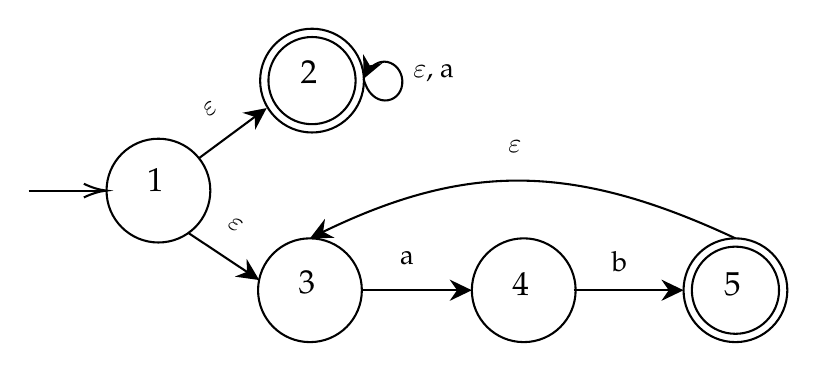
\begin{tikzpicture}[x=0.75pt,y=0.75pt,yscale=-1,xscale=1]
%uncomment if require: \path (0,174); %set diagram left start at 0, and has height of 174

%Shape: Circle [id:dp6332800579810671] 
\draw   (221,36) .. controls (221,22.19) and (232.19,11) .. (246,11) .. controls (259.81,11) and (271,22.19) .. (271,36) .. controls (271,49.81) and (259.81,61) .. (246,61) .. controls (232.19,61) and (221,49.81) .. (221,36) -- cycle ;
%Curve Lines [id:da9468975555842336] 
\draw    (270.86,35.14) .. controls (274.46,49.64) and (288.46,47.64) .. (289.46,37.64) .. controls (290.39,28.29) and (279.09,21.56) .. (272.22,32.58) ;
\draw [shift={(270.86,35.14)}, rotate = 294.47] [fill={rgb, 255:red, 0; green, 0; blue, 0 }  ][line width=0.08]  [draw opacity=0] (10.72,-5.15) -- (0,0) -- (10.72,5.15) -- (7.12,0) -- cycle    ;
%Shape: Circle [id:dp9803411326519775] 
\draw   (220,137) .. controls (220,123.19) and (231.19,112) .. (245,112) .. controls (258.81,112) and (270,123.19) .. (270,137) .. controls (270,150.81) and (258.81,162) .. (245,162) .. controls (231.19,162) and (220,150.81) .. (220,137) -- cycle ;
%Shape: Circle [id:dp7461557307413222] 
\draw   (323,137) .. controls (323,123.19) and (334.19,112) .. (348,112) .. controls (361.81,112) and (373,123.19) .. (373,137) .. controls (373,150.81) and (361.81,162) .. (348,162) .. controls (334.19,162) and (323,150.81) .. (323,137) -- cycle ;
%Straight Lines [id:da7188746919776186] 
\draw    (270,137) -- (320,137) ;
\draw [shift={(323,137)}, rotate = 180] [fill={rgb, 255:red, 0; green, 0; blue, 0 }  ][line width=0.08]  [draw opacity=0] (10.72,-5.15) -- (0,0) -- (10.72,5.15) -- (7.12,0) -- cycle    ;
%Shape: Circle [id:dp03739142514118732] 
\draw   (425,137) .. controls (425,123.19) and (436.19,112) .. (450,112) .. controls (463.81,112) and (475,123.19) .. (475,137) .. controls (475,150.81) and (463.81,162) .. (450,162) .. controls (436.19,162) and (425,150.81) .. (425,137) -- cycle ;
%Straight Lines [id:da2664871268638893] 
\draw    (372,137) -- (422,137) ;
\draw [shift={(425,137)}, rotate = 180] [fill={rgb, 255:red, 0; green, 0; blue, 0 }  ][line width=0.08]  [draw opacity=0] (10.72,-5.15) -- (0,0) -- (10.72,5.15) -- (7.12,0) -- cycle    ;
%Shape: Circle [id:dp4855024547701494] 
\draw   (147,89) .. controls (147,75.19) and (158.19,64) .. (172,64) .. controls (185.81,64) and (197,75.19) .. (197,89) .. controls (197,102.81) and (185.81,114) .. (172,114) .. controls (158.19,114) and (147,102.81) .. (147,89) -- cycle ;
%Straight Lines [id:da4713456738805095] 
\draw    (109.5,89) -- (145,89) ;
\draw [shift={(147,89)}, rotate = 180] [color={rgb, 255:red, 0; green, 0; blue, 0 }  ][line width=0.75]    (10.93,-3.29) .. controls (6.95,-1.4) and (3.31,-0.3) .. (0,0) .. controls (3.31,0.3) and (6.95,1.4) .. (10.93,3.29)   ;
%Straight Lines [id:da1984076573956659] 
\draw    (191.5,73.4) -- (221.72,51.04) ;
\draw [shift={(224.13,49.26)}, rotate = 503.5] [fill={rgb, 255:red, 0; green, 0; blue, 0 }  ][line width=0.08]  [draw opacity=0] (10.72,-5.15) -- (0,0) -- (10.72,5.15) -- (7.12,0) -- cycle    ;
%Straight Lines [id:da5265969920815687] 
\draw    (186.75,109.62) -- (218.06,130.42) ;
\draw [shift={(220.56,132.09)}, rotate = 213.61] [fill={rgb, 255:red, 0; green, 0; blue, 0 }  ][line width=0.08]  [draw opacity=0] (10.72,-5.15) -- (0,0) -- (10.72,5.15) -- (7.12,0) -- cycle    ;
%Shape: Circle [id:dp4316346314364601] 
\draw   (225,36) .. controls (225,24.4) and (234.4,15) .. (246,15) .. controls (257.6,15) and (267,24.4) .. (267,36) .. controls (267,47.6) and (257.6,57) .. (246,57) .. controls (234.4,57) and (225,47.6) .. (225,36) -- cycle ;
%Shape: Circle [id:dp5198414150675785] 
\draw   (429,137) .. controls (429,125.4) and (438.4,116) .. (450,116) .. controls (461.6,116) and (471,125.4) .. (471,137) .. controls (471,148.6) and (461.6,158) .. (450,158) .. controls (438.4,158) and (429,148.6) .. (429,137) -- cycle ;
%Curve Lines [id:da6905943582577521] 
\draw    (450,112) .. controls (370.3,74.78) and (318.54,75.38) .. (247.17,110.91) ;
\draw [shift={(245,112)}, rotate = 333.21000000000004] [fill={rgb, 255:red, 0; green, 0; blue, 0 }  ][line width=0.08]  [draw opacity=0] (10.72,-5.15) -- (0,0) -- (10.72,5.15) -- (7.12,0) -- cycle    ;

% Text Node
\draw (239,25) node [anchor=north west][inner sep=0.75pt]  [font=\large] [align=left] {2};
% Text Node
\draw (293.46,26.63) node [anchor=north west][inner sep=0.75pt]  [rotate=-0.57] [align=left] {$\displaystyle \varepsilon $, a};
% Text Node
\draw (238,126) node [anchor=north west][inner sep=0.75pt]  [font=\large] [align=left] {3};
% Text Node
\draw (341,127) node [anchor=north west][inner sep=0.75pt]  [font=\large] [align=left] {4};
% Text Node
\draw (287,117) node [anchor=north west][inner sep=0.75pt]   [align=left] {a};
% Text Node
\draw (443,127) node [anchor=north west][inner sep=0.75pt]  [font=\large] [align=left] {5};
% Text Node
\draw (389,117) node [anchor=north west][inner sep=0.75pt]   [align=left] {b};
% Text Node
\draw (190.47,48.8) node [anchor=north west][inner sep=0.75pt]  [rotate=-321.8] [align=left] {$\displaystyle \varepsilon $};
% Text Node
\draw (207.53,99.28) node [anchor=north west][inner sep=0.75pt]  [rotate=-31.91] [align=left] {$\displaystyle \varepsilon $};
% Text Node
\draw (339.13,63.5) node [anchor=north west][inner sep=0.75pt]  [rotate=-0.67] [align=left] {$\displaystyle \varepsilon $};
% Text Node
\draw (165,77) node [anchor=north west][inner sep=0.75pt]  [font=\large] [align=left] {1};


\end{tikzpicture}


\begin{prob}\end{prob}

\begin{enumerate}[label=(\alph*)]

\item
The primary differences between NFA and DFA are as follows
\begin{enumerate}[label=\arabic*.]
\item There are multiple possible out arrows for a single value
\item $\varepsilon$ is allowed on an arrow
\item Some values lead to $\varnothing$ / they don't lead anywhere.
\end{enumerate}

\item
The primary difference between GNFA and NFA is that GNFA uses regular expressions on arrows, 
whereas NFA does not.

\end{enumerate}

\newpage

\begin{prob}\end{prob}

\begin{enumerate}[label=(\alph*)]

\item
\begin{enumerate}[label=\arabic*.]

\item
\textbf{NFA to GNFA}


\tikzset{every picture/.style={line width=0.75pt}} %set default line width to 0.75pt        

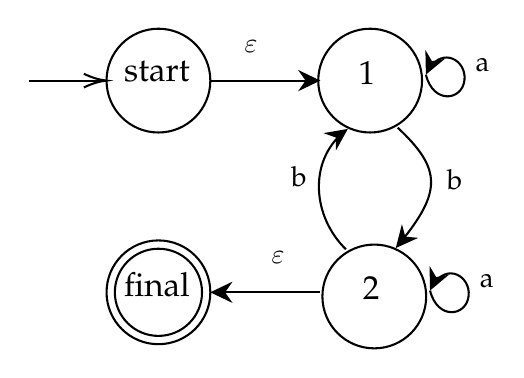
\begin{tikzpicture}[x=0.75pt,y=0.75pt,yscale=-1,xscale=1]
%uncomment if require: \path (0,184); %set diagram left start at 0, and has height of 184

%Shape: Circle [id:dp4399582060172538] 
\draw   (155,41) .. controls (155,27.19) and (166.19,16) .. (180,16) .. controls (193.81,16) and (205,27.19) .. (205,41) .. controls (205,54.81) and (193.81,66) .. (180,66) .. controls (166.19,66) and (155,54.81) .. (155,41) -- cycle ;
%Curve Lines [id:da7162815099620423] 
\draw    (206.86,38.14) .. controls (210.46,52.64) and (224.46,50.64) .. (225.46,40.64) .. controls (226.39,31.29) and (215.09,24.56) .. (208.22,35.58) ;
\draw [shift={(206.86,38.14)}, rotate = 294.47] [fill={rgb, 255:red, 0; green, 0; blue, 0 }  ][line width=0.08]  [draw opacity=0] (10.72,-5.15) -- (0,0) -- (10.72,5.15) -- (7.12,0) -- cycle    ;
%Shape: Circle [id:dp8199620206801059] 
\draw   (53,41) .. controls (53,27.19) and (64.19,16) .. (78,16) .. controls (91.81,16) and (103,27.19) .. (103,41) .. controls (103,54.81) and (91.81,66) .. (78,66) .. controls (64.19,66) and (53,54.81) .. (53,41) -- cycle ;
%Straight Lines [id:da5007258032913255] 
\draw    (15.5,41) -- (51,41) ;
\draw [shift={(53,41)}, rotate = 180] [color={rgb, 255:red, 0; green, 0; blue, 0 }  ][line width=0.75]    (10.93,-3.29) .. controls (6.95,-1.4) and (3.31,-0.3) .. (0,0) .. controls (3.31,0.3) and (6.95,1.4) .. (10.93,3.29)   ;
%Straight Lines [id:da1610232969723413] 
\draw    (103,41) -- (153,41) ;
\draw [shift={(156,41)}, rotate = 180] [fill={rgb, 255:red, 0; green, 0; blue, 0 }  ][line width=0.08]  [draw opacity=0] (10.72,-5.15) -- (0,0) -- (10.72,5.15) -- (7.12,0) -- cycle    ;
%Shape: Circle [id:dp8634067085317565] 
\draw   (157,145) .. controls (157,131.19) and (168.19,120) .. (182,120) .. controls (195.81,120) and (207,131.19) .. (207,145) .. controls (207,158.81) and (195.81,170) .. (182,170) .. controls (168.19,170) and (157,158.81) .. (157,145) -- cycle ;
%Curve Lines [id:da8803862200785482] 
\draw    (208.86,142.14) .. controls (212.46,156.64) and (226.46,154.64) .. (227.46,144.64) .. controls (228.39,135.29) and (217.09,128.56) .. (210.22,139.58) ;
\draw [shift={(208.86,142.14)}, rotate = 294.47] [fill={rgb, 255:red, 0; green, 0; blue, 0 }  ][line width=0.08]  [draw opacity=0] (10.72,-5.15) -- (0,0) -- (10.72,5.15) -- (7.12,0) -- cycle    ;
%Curve Lines [id:da24057158939454282] 
\draw    (193.26,63.66) .. controls (214.4,83.49) and (214.77,94.44) .. (194,119.68) ;
\draw [shift={(192.36,121.65)}, rotate = 310.06] [fill={rgb, 255:red, 0; green, 0; blue, 0 }  ][line width=0.08]  [draw opacity=0] (10.72,-5.15) -- (0,0) -- (10.72,5.15) -- (7.12,0) -- cycle    ;
%Curve Lines [id:da23977895742246536] 
\draw    (168.34,122.28) .. controls (152.26,106.66) and (150.18,80.21) .. (167.04,65.99) ;
\draw [shift={(169.24,64.28)}, rotate = 504.51] [fill={rgb, 255:red, 0; green, 0; blue, 0 }  ][line width=0.08]  [draw opacity=0] (10.72,-5.15) -- (0,0) -- (10.72,5.15) -- (7.12,0) -- cycle    ;
%Shape: Circle [id:dp7594811546626297] 
\draw   (53,143) .. controls (53,129.19) and (64.19,118) .. (78,118) .. controls (91.81,118) and (103,129.19) .. (103,143) .. controls (103,156.81) and (91.81,168) .. (78,168) .. controls (64.19,168) and (53,156.81) .. (53,143) -- cycle ;
%Straight Lines [id:da9352941256796419] 
\draw    (156,143) -- (106,143) ;
\draw [shift={(103,143)}, rotate = 360] [fill={rgb, 255:red, 0; green, 0; blue, 0 }  ][line width=0.08]  [draw opacity=0] (10.72,-5.15) -- (0,0) -- (10.72,5.15) -- (7.12,0) -- cycle    ;
%Shape: Circle [id:dp19714558386608405] 
\draw   (57,143) .. controls (57,131.4) and (66.4,122) .. (78,122) .. controls (89.6,122) and (99,131.4) .. (99,143) .. controls (99,154.6) and (89.6,164) .. (78,164) .. controls (66.4,164) and (57,154.6) .. (57,143) -- cycle ;

% Text Node
\draw (173,30) node [anchor=north west][inner sep=0.75pt]  [font=\large] [align=left] {1};
% Text Node
\draw (229.33,28.79) node [anchor=north west][inner sep=0.75pt]  [rotate=-359.74] [align=left] {a};
% Text Node
\draw (60,30) node [anchor=north west][inner sep=0.75pt]  [font=\large] [align=left] {start};
% Text Node
\draw (118,20) node [anchor=north west][inner sep=0.75pt]   [align=left] {$\displaystyle \varepsilon $};
% Text Node
\draw (175,134) node [anchor=north west][inner sep=0.75pt]  [font=\large] [align=left] {2};
% Text Node
\draw (231.33,132.79) node [anchor=north west][inner sep=0.75pt]  [rotate=-359.74] [align=left] {a};
% Text Node
\draw (215.7,81.99) node [anchor=north west][inner sep=0.75pt]  [rotate=-1.05] [align=left] {b};
% Text Node
\draw (140.6,80.89) node [anchor=north west][inner sep=0.75pt]  [rotate=-0.31] [align=left] {b};
% Text Node
\draw (60,132) node [anchor=north west][inner sep=0.75pt]  [font=\large] [align=left] {final};
% Text Node
\draw (131,122) node [anchor=north west][inner sep=0.75pt]   [align=left] {$\displaystyle \varepsilon $};


\end{tikzpicture}

\item
\textbf{Strip 1}



\tikzset{every picture/.style={line width=0.75pt}} %set default line width to 0.75pt        

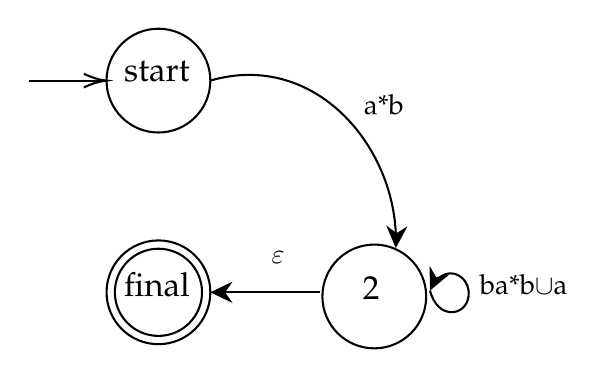
\begin{tikzpicture}[x=0.75pt,y=0.75pt,yscale=-1,xscale=1]
%uncomment if require: \path (0,182); %set diagram left start at 0, and has height of 182

%Shape: Circle [id:dp8821658490377933] 
\draw   (56,42) .. controls (56,28.19) and (67.19,17) .. (81,17) .. controls (94.81,17) and (106,28.19) .. (106,42) .. controls (106,55.81) and (94.81,67) .. (81,67) .. controls (67.19,67) and (56,55.81) .. (56,42) -- cycle ;
%Straight Lines [id:da2684112133913743] 
\draw    (18.5,42) -- (54,42) ;
\draw [shift={(56,42)}, rotate = 180] [color={rgb, 255:red, 0; green, 0; blue, 0 }  ][line width=0.75]    (10.93,-3.29) .. controls (6.95,-1.4) and (3.31,-0.3) .. (0,0) .. controls (3.31,0.3) and (6.95,1.4) .. (10.93,3.29)   ;
%Shape: Circle [id:dp7192939088422887] 
\draw   (160,146) .. controls (160,132.19) and (171.19,121) .. (185,121) .. controls (198.81,121) and (210,132.19) .. (210,146) .. controls (210,159.81) and (198.81,171) .. (185,171) .. controls (171.19,171) and (160,159.81) .. (160,146) -- cycle ;
%Curve Lines [id:da038424125975401235] 
\draw    (211.86,143.14) .. controls (215.46,157.64) and (229.46,155.64) .. (230.46,145.64) .. controls (231.39,136.29) and (220.09,129.56) .. (213.22,140.58) ;
\draw [shift={(211.86,143.14)}, rotate = 294.47] [fill={rgb, 255:red, 0; green, 0; blue, 0 }  ][line width=0.08]  [draw opacity=0] (10.72,-5.15) -- (0,0) -- (10.72,5.15) -- (7.12,0) -- cycle    ;
%Curve Lines [id:da949192435967368] 
\draw    (106,42) .. controls (156.47,27.3) and (195.9,74.07) .. (195.43,119.85) ;
\draw [shift={(195.36,122.65)}, rotate = 272.63] [fill={rgb, 255:red, 0; green, 0; blue, 0 }  ][line width=0.08]  [draw opacity=0] (10.72,-5.15) -- (0,0) -- (10.72,5.15) -- (7.12,0) -- cycle    ;
%Shape: Circle [id:dp5346912012374245] 
\draw   (56,144) .. controls (56,130.19) and (67.19,119) .. (81,119) .. controls (94.81,119) and (106,130.19) .. (106,144) .. controls (106,157.81) and (94.81,169) .. (81,169) .. controls (67.19,169) and (56,157.81) .. (56,144) -- cycle ;
%Straight Lines [id:da3037393523203442] 
\draw    (159,144) -- (109,144) ;
\draw [shift={(106,144)}, rotate = 360] [fill={rgb, 255:red, 0; green, 0; blue, 0 }  ][line width=0.08]  [draw opacity=0] (10.72,-5.15) -- (0,0) -- (10.72,5.15) -- (7.12,0) -- cycle    ;
%Shape: Circle [id:dp7846846644554537] 
\draw   (60,144) .. controls (60,132.4) and (69.4,123) .. (81,123) .. controls (92.6,123) and (102,132.4) .. (102,144) .. controls (102,155.6) and (92.6,165) .. (81,165) .. controls (69.4,165) and (60,155.6) .. (60,144) -- cycle ;

% Text Node
\draw (63,31) node [anchor=north west][inner sep=0.75pt]  [font=\large] [align=left] {start};
% Text Node
\draw (178,135) node [anchor=north west][inner sep=0.75pt]  [font=\large] [align=left] {2};
% Text Node
\draw (234.33,133.79) node [anchor=north west][inner sep=0.75pt]  [rotate=-359.74] [align=left] {ba*b$\displaystyle \cup $a};
% Text Node
\draw (178.7,46.99) node [anchor=north west][inner sep=0.75pt]  [rotate=-1.05] [align=left] {a*b};
% Text Node
\draw (63,133) node [anchor=north west][inner sep=0.75pt]  [font=\large] [align=left] {final};
% Text Node
\draw (134,123) node [anchor=north west][inner sep=0.75pt]   [align=left] {$\displaystyle \varepsilon $};


\end{tikzpicture}


\item
\textbf{Strip 2}



\tikzset{every picture/.style={line width=0.75pt}} %set default line width to 0.75pt        

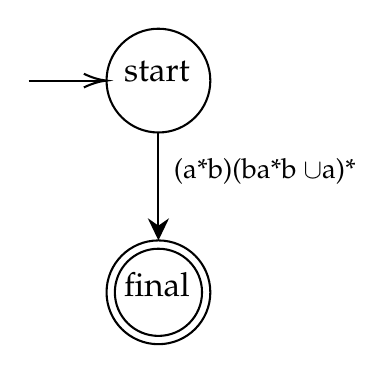
\begin{tikzpicture}[x=0.75pt,y=0.75pt,yscale=-1,xscale=1]
%uncomment if require: \path (0,182); %set diagram left start at 0, and has height of 182

%Shape: Circle [id:dp8012899459358327] 
\draw   (57,45) .. controls (57,31.19) and (68.19,20) .. (82,20) .. controls (95.81,20) and (107,31.19) .. (107,45) .. controls (107,58.81) and (95.81,70) .. (82,70) .. controls (68.19,70) and (57,58.81) .. (57,45) -- cycle ;
%Straight Lines [id:da2300760703732152] 
\draw    (19.5,45) -- (55,45) ;
\draw [shift={(57,45)}, rotate = 180] [color={rgb, 255:red, 0; green, 0; blue, 0 }  ][line width=0.75]    (10.93,-3.29) .. controls (6.95,-1.4) and (3.31,-0.3) .. (0,0) .. controls (3.31,0.3) and (6.95,1.4) .. (10.93,3.29)   ;
%Shape: Circle [id:dp45165672541812696] 
\draw   (57,147) .. controls (57,133.19) and (68.19,122) .. (82,122) .. controls (95.81,122) and (107,133.19) .. (107,147) .. controls (107,160.81) and (95.81,172) .. (82,172) .. controls (68.19,172) and (57,160.81) .. (57,147) -- cycle ;
%Shape: Circle [id:dp3339649363965109] 
\draw   (61,147) .. controls (61,135.4) and (70.4,126) .. (82,126) .. controls (93.6,126) and (103,135.4) .. (103,147) .. controls (103,158.6) and (93.6,168) .. (82,168) .. controls (70.4,168) and (61,158.6) .. (61,147) -- cycle ;
%Straight Lines [id:da7766152456837094] 
\draw    (82,70) -- (82,119) ;
\draw [shift={(82,122)}, rotate = 270] [fill={rgb, 255:red, 0; green, 0; blue, 0 }  ][line width=0.08]  [draw opacity=0] (10.72,-5.15) -- (0,0) -- (10.72,5.15) -- (7.12,0) -- cycle    ;

% Text Node
\draw (64,34) node [anchor=north west][inner sep=0.75pt]  [font=\large] [align=left] {start};
% Text Node
\draw (64,136) node [anchor=north west][inner sep=0.75pt]  [font=\large] [align=left] {final};
% Text Node
\draw (88,81) node [anchor=north west][inner sep=0.75pt]   [align=left] {(a*b)(ba*b $\displaystyle \cup $a)*};


\end{tikzpicture}

\end{enumerate}

\newpage

\item

\begin{enumerate}[label=\arabic*.]

\item
\textbf{NFA to GNFA}



\tikzset{every picture/.style={line width=0.75pt}} %set default line width to 0.75pt        

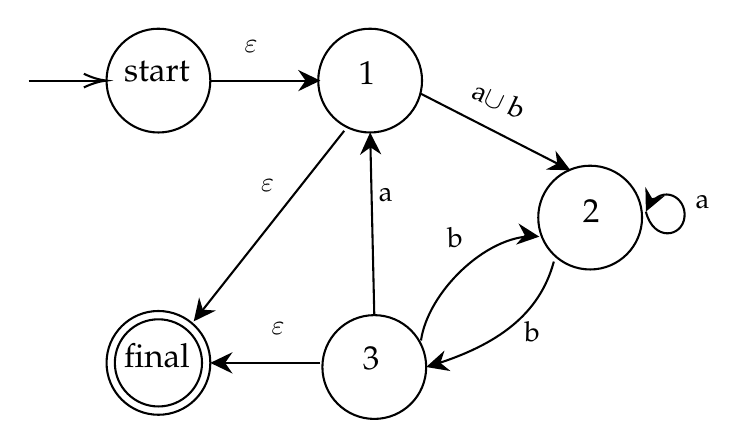
\begin{tikzpicture}[x=0.75pt,y=0.75pt,yscale=-1,xscale=1]
%uncomment if require: \path (0,226); %set diagram left start at 0, and has height of 226

%Shape: Circle [id:dp014885445218258742] 
\draw   (161,43) .. controls (161,29.19) and (172.19,18) .. (186,18) .. controls (199.81,18) and (211,29.19) .. (211,43) .. controls (211,56.81) and (199.81,68) .. (186,68) .. controls (172.19,68) and (161,56.81) .. (161,43) -- cycle ;
%Shape: Circle [id:dp7663908677482769] 
\draw   (59,43) .. controls (59,29.19) and (70.19,18) .. (84,18) .. controls (97.81,18) and (109,29.19) .. (109,43) .. controls (109,56.81) and (97.81,68) .. (84,68) .. controls (70.19,68) and (59,56.81) .. (59,43) -- cycle ;
%Straight Lines [id:da03722913295401309] 
\draw    (21.5,43) -- (57,43) ;
\draw [shift={(59,43)}, rotate = 180] [color={rgb, 255:red, 0; green, 0; blue, 0 }  ][line width=0.75]    (10.93,-3.29) .. controls (6.95,-1.4) and (3.31,-0.3) .. (0,0) .. controls (3.31,0.3) and (6.95,1.4) .. (10.93,3.29)   ;
%Straight Lines [id:da887610695586734] 
\draw    (109,43) -- (159,43) ;
\draw [shift={(162,43)}, rotate = 180] [fill={rgb, 255:red, 0; green, 0; blue, 0 }  ][line width=0.08]  [draw opacity=0] (10.72,-5.15) -- (0,0) -- (10.72,5.15) -- (7.12,0) -- cycle    ;
%Shape: Circle [id:dp22327933627285046] 
\draw   (163,181) .. controls (163,167.19) and (174.19,156) .. (188,156) .. controls (201.81,156) and (213,167.19) .. (213,181) .. controls (213,194.81) and (201.81,206) .. (188,206) .. controls (174.19,206) and (163,194.81) .. (163,181) -- cycle ;
%Curve Lines [id:da3334923596398114] 
\draw    (274.5,130.2) .. controls (267.68,155.55) and (247.54,170.44) .. (215.49,180.26) ;
\draw [shift={(213,181)}, rotate = 343.69] [fill={rgb, 255:red, 0; green, 0; blue, 0 }  ][line width=0.08]  [draw opacity=0] (10.72,-5.15) -- (0,0) -- (10.72,5.15) -- (7.12,0) -- cycle    ;
%Curve Lines [id:da4627773623783942] 
\draw    (210.5,168.2) .. controls (213.81,145.02) and (241.64,117.69) .. (264.65,118.01) ;
\draw [shift={(267.5,118.2)}, rotate = 186.79] [fill={rgb, 255:red, 0; green, 0; blue, 0 }  ][line width=0.08]  [draw opacity=0] (10.72,-5.15) -- (0,0) -- (10.72,5.15) -- (7.12,0) -- cycle    ;
%Shape: Circle [id:dp7277320145729371] 
\draw   (59,179) .. controls (59,165.19) and (70.19,154) .. (84,154) .. controls (97.81,154) and (109,165.19) .. (109,179) .. controls (109,192.81) and (97.81,204) .. (84,204) .. controls (70.19,204) and (59,192.81) .. (59,179) -- cycle ;
%Straight Lines [id:da8845379568033749] 
\draw    (162,179) -- (112,179) ;
\draw [shift={(109,179)}, rotate = 360] [fill={rgb, 255:red, 0; green, 0; blue, 0 }  ][line width=0.08]  [draw opacity=0] (10.72,-5.15) -- (0,0) -- (10.72,5.15) -- (7.12,0) -- cycle    ;
%Shape: Circle [id:dp898655860779074] 
\draw   (63,179) .. controls (63,167.4) and (72.4,158) .. (84,158) .. controls (95.6,158) and (105,167.4) .. (105,179) .. controls (105,190.6) and (95.6,200) .. (84,200) .. controls (72.4,200) and (63,190.6) .. (63,179) -- cycle ;
%Shape: Circle [id:dp6647116893707181] 
\draw   (267,109) .. controls (267,95.19) and (278.19,84) .. (292,84) .. controls (305.81,84) and (317,95.19) .. (317,109) .. controls (317,122.81) and (305.81,134) .. (292,134) .. controls (278.19,134) and (267,122.81) .. (267,109) -- cycle ;
%Curve Lines [id:da5246514045971398] 
\draw    (318.86,106.14) .. controls (322.46,120.64) and (336.46,118.64) .. (337.46,108.64) .. controls (338.39,99.29) and (327.09,92.56) .. (320.22,103.58) ;
\draw [shift={(318.86,106.14)}, rotate = 294.47] [fill={rgb, 255:red, 0; green, 0; blue, 0 }  ][line width=0.08]  [draw opacity=0] (10.72,-5.15) -- (0,0) -- (10.72,5.15) -- (7.12,0) -- cycle    ;
%Straight Lines [id:da3371733675223041] 
\draw    (210.11,49.16) -- (279.83,84.83) ;
\draw [shift={(282.5,86.2)}, rotate = 207.1] [fill={rgb, 255:red, 0; green, 0; blue, 0 }  ][line width=0.08]  [draw opacity=0] (10.72,-5.15) -- (0,0) -- (10.72,5.15) -- (7.12,0) -- cycle    ;
%Straight Lines [id:da2399242492803828] 
\draw    (173.5,67.2) -- (102.86,156.65) ;
\draw [shift={(101,159)}, rotate = 308.3] [fill={rgb, 255:red, 0; green, 0; blue, 0 }  ][line width=0.08]  [draw opacity=0] (10.72,-5.15) -- (0,0) -- (10.72,5.15) -- (7.12,0) -- cycle    ;
%Straight Lines [id:da7784085557442126] 
\draw    (188,156) -- (186.07,71) ;
\draw [shift={(186,68)}, rotate = 448.7] [fill={rgb, 255:red, 0; green, 0; blue, 0 }  ][line width=0.08]  [draw opacity=0] (10.72,-5.15) -- (0,0) -- (10.72,5.15) -- (7.12,0) -- cycle    ;

% Text Node
\draw (179,32) node [anchor=north west][inner sep=0.75pt]  [font=\large] [align=left] {1};
% Text Node
\draw (66,32) node [anchor=north west][inner sep=0.75pt]  [font=\large] [align=left] {start};
% Text Node
\draw (124,22) node [anchor=north west][inner sep=0.75pt]   [align=left] {$\displaystyle \varepsilon $};
% Text Node
\draw (181,170) node [anchor=north west][inner sep=0.75pt]  [font=\large] [align=left] {3};
% Text Node
\draw (259.03,157.66) node [anchor=north west][inner sep=0.75pt]  [rotate=-1.33] [align=left] {b};
% Text Node
\draw (221.63,112.45) node [anchor=north west][inner sep=0.75pt]  [rotate=-359.11] [align=left] {b};
% Text Node
\draw (66,168) node [anchor=north west][inner sep=0.75pt]  [font=\large] [align=left] {final};
% Text Node
\draw (137,158) node [anchor=north west][inner sep=0.75pt]   [align=left] {$\displaystyle \varepsilon $};
% Text Node
\draw (341.33,96.79) node [anchor=north west][inner sep=0.75pt]  [rotate=-359.74] [align=left] {a};
% Text Node
\draw (287,99) node [anchor=north west][inner sep=0.75pt]  [font=\large] [align=left] {2};
% Text Node
\draw (237.74,40.17) node [anchor=north west][inner sep=0.75pt]  [rotate=-25.38] [align=left] {a$\displaystyle \cup $ b};
% Text Node
\draw (132,89) node [anchor=north west][inner sep=0.75pt]   [align=left] {$\displaystyle \varepsilon $};
% Text Node
\draw (188.63,93.45) node [anchor=north west][inner sep=0.75pt]  [rotate=-359.11] [align=left] {a};


\end{tikzpicture}


\item
\textbf{Strip 1}


\tikzset{every picture/.style={line width=0.75pt}} %set default line width to 0.75pt        

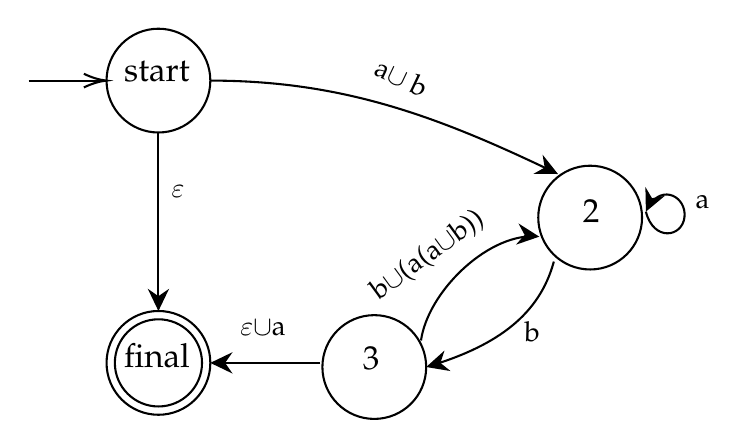
\begin{tikzpicture}[x=0.75pt,y=0.75pt,yscale=-1,xscale=1]
%uncomment if require: \path (0,223); %set diagram left start at 0, and has height of 223

%Shape: Circle [id:dp37352155173333434] 
\draw   (56,42) .. controls (56,28.19) and (67.19,17) .. (81,17) .. controls (94.81,17) and (106,28.19) .. (106,42) .. controls (106,55.81) and (94.81,67) .. (81,67) .. controls (67.19,67) and (56,55.81) .. (56,42) -- cycle ;
%Straight Lines [id:da9724085836425722] 
\draw    (18.5,42) -- (54,42) ;
\draw [shift={(56,42)}, rotate = 180] [color={rgb, 255:red, 0; green, 0; blue, 0 }  ][line width=0.75]    (10.93,-3.29) .. controls (6.95,-1.4) and (3.31,-0.3) .. (0,0) .. controls (3.31,0.3) and (6.95,1.4) .. (10.93,3.29)   ;
%Shape: Circle [id:dp7348642306487412] 
\draw   (160,180) .. controls (160,166.19) and (171.19,155) .. (185,155) .. controls (198.81,155) and (210,166.19) .. (210,180) .. controls (210,193.81) and (198.81,205) .. (185,205) .. controls (171.19,205) and (160,193.81) .. (160,180) -- cycle ;
%Curve Lines [id:da07463849948020695] 
\draw    (271.5,129.2) .. controls (264.68,154.55) and (244.54,169.44) .. (212.49,179.26) ;
\draw [shift={(210,180)}, rotate = 343.69] [fill={rgb, 255:red, 0; green, 0; blue, 0 }  ][line width=0.08]  [draw opacity=0] (10.72,-5.15) -- (0,0) -- (10.72,5.15) -- (7.12,0) -- cycle    ;
%Curve Lines [id:da18767721913223623] 
\draw    (207.5,167.2) .. controls (210.81,144.02) and (238.64,116.69) .. (261.65,117.01) ;
\draw [shift={(264.5,117.2)}, rotate = 186.79] [fill={rgb, 255:red, 0; green, 0; blue, 0 }  ][line width=0.08]  [draw opacity=0] (10.72,-5.15) -- (0,0) -- (10.72,5.15) -- (7.12,0) -- cycle    ;
%Shape: Circle [id:dp42156246722795787] 
\draw   (56,178) .. controls (56,164.19) and (67.19,153) .. (81,153) .. controls (94.81,153) and (106,164.19) .. (106,178) .. controls (106,191.81) and (94.81,203) .. (81,203) .. controls (67.19,203) and (56,191.81) .. (56,178) -- cycle ;
%Straight Lines [id:da17996364363748296] 
\draw    (159,178) -- (109,178) ;
\draw [shift={(106,178)}, rotate = 360] [fill={rgb, 255:red, 0; green, 0; blue, 0 }  ][line width=0.08]  [draw opacity=0] (10.72,-5.15) -- (0,0) -- (10.72,5.15) -- (7.12,0) -- cycle    ;
%Shape: Circle [id:dp48180726109062944] 
\draw   (60,178) .. controls (60,166.4) and (69.4,157) .. (81,157) .. controls (92.6,157) and (102,166.4) .. (102,178) .. controls (102,189.6) and (92.6,199) .. (81,199) .. controls (69.4,199) and (60,189.6) .. (60,178) -- cycle ;
%Shape: Circle [id:dp7405108105587599] 
\draw   (264,108) .. controls (264,94.19) and (275.19,83) .. (289,83) .. controls (302.81,83) and (314,94.19) .. (314,108) .. controls (314,121.81) and (302.81,133) .. (289,133) .. controls (275.19,133) and (264,121.81) .. (264,108) -- cycle ;
%Curve Lines [id:da7518069775317919] 
\draw    (315.86,105.14) .. controls (319.46,119.64) and (333.46,117.64) .. (334.46,107.64) .. controls (335.39,98.29) and (324.09,91.56) .. (317.22,102.58) ;
\draw [shift={(315.86,105.14)}, rotate = 294.47] [fill={rgb, 255:red, 0; green, 0; blue, 0 }  ][line width=0.08]  [draw opacity=0] (10.72,-5.15) -- (0,0) -- (10.72,5.15) -- (7.12,0) -- cycle    ;
%Curve Lines [id:da8314659473211015] 
\draw    (106,42) .. controls (168.55,42) and (214.12,58.49) .. (270.9,85.75) ;
\draw [shift={(273.5,87)}, rotate = 205.77] [fill={rgb, 255:red, 0; green, 0; blue, 0 }  ][line width=0.08]  [draw opacity=0] (10.72,-5.15) -- (0,0) -- (10.72,5.15) -- (7.12,0) -- cycle    ;
%Straight Lines [id:da13507178315648738] 
\draw    (81,67) -- (81,150) ;
\draw [shift={(81,153)}, rotate = 270] [fill={rgb, 255:red, 0; green, 0; blue, 0 }  ][line width=0.08]  [draw opacity=0] (10.72,-5.15) -- (0,0) -- (10.72,5.15) -- (7.12,0) -- cycle    ;

% Text Node
\draw (63,31) node [anchor=north west][inner sep=0.75pt]  [font=\large] [align=left] {start};
% Text Node
\draw (178,169) node [anchor=north west][inner sep=0.75pt]  [font=\large] [align=left] {3};
% Text Node
\draw (256.03,156.66) node [anchor=north west][inner sep=0.75pt]  [rotate=-1.33] [align=left] {b};
% Text Node
\draw (179.29,139.55) node [anchor=north west][inner sep=0.75pt]  [rotate=-323.92] [align=left] {b$\displaystyle \cup $(a(a$\displaystyle \cup $b))};
% Text Node
\draw (63,167) node [anchor=north west][inner sep=0.75pt]  [font=\large] [align=left] {final};
% Text Node
\draw (119,156) node [anchor=north west][inner sep=0.75pt]   [align=left] {$\displaystyle \varepsilon \cup $a};
% Text Node
\draw (338.33,95.79) node [anchor=north west][inner sep=0.75pt]  [rotate=-359.74] [align=left] {a};
% Text Node
\draw (284,98) node [anchor=north west][inner sep=0.75pt]  [font=\large] [align=left] {2};
% Text Node
\draw (187.74,28.17) node [anchor=north west][inner sep=0.75pt]  [rotate=-25.38] [align=left] {a$\displaystyle \cup $ b};
% Text Node
\draw (85.84,91.22) node [anchor=north west][inner sep=0.75pt]  [rotate=-359.61] [align=left] {$\displaystyle \varepsilon $};


\end{tikzpicture}


\item
\textbf{Strip 2}



\tikzset{every picture/.style={line width=0.75pt}} %set default line width to 0.75pt        

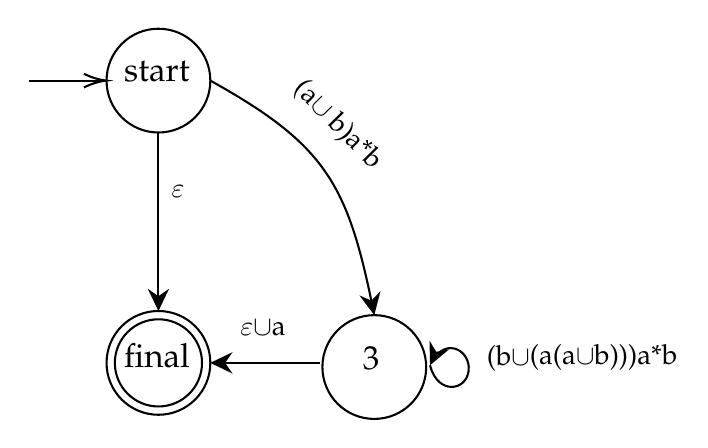
\begin{tikzpicture}[x=0.75pt,y=0.75pt,yscale=-1,xscale=1]
%uncomment if require: \path (0,227); %set diagram left start at 0, and has height of 227

%Shape: Circle [id:dp561752195878239] 
\draw   (53,46) .. controls (53,32.19) and (64.19,21) .. (78,21) .. controls (91.81,21) and (103,32.19) .. (103,46) .. controls (103,59.81) and (91.81,71) .. (78,71) .. controls (64.19,71) and (53,59.81) .. (53,46) -- cycle ;
%Straight Lines [id:da15648285395389205] 
\draw    (15.5,46) -- (51,46) ;
\draw [shift={(53,46)}, rotate = 180] [color={rgb, 255:red, 0; green, 0; blue, 0 }  ][line width=0.75]    (10.93,-3.29) .. controls (6.95,-1.4) and (3.31,-0.3) .. (0,0) .. controls (3.31,0.3) and (6.95,1.4) .. (10.93,3.29)   ;
%Shape: Circle [id:dp28079544014299085] 
\draw   (157,184) .. controls (157,170.19) and (168.19,159) .. (182,159) .. controls (195.81,159) and (207,170.19) .. (207,184) .. controls (207,197.81) and (195.81,209) .. (182,209) .. controls (168.19,209) and (157,197.81) .. (157,184) -- cycle ;
%Shape: Circle [id:dp7219088223018555] 
\draw   (53,182) .. controls (53,168.19) and (64.19,157) .. (78,157) .. controls (91.81,157) and (103,168.19) .. (103,182) .. controls (103,195.81) and (91.81,207) .. (78,207) .. controls (64.19,207) and (53,195.81) .. (53,182) -- cycle ;
%Straight Lines [id:da3987382540168847] 
\draw    (156,182) -- (106,182) ;
\draw [shift={(103,182)}, rotate = 360] [fill={rgb, 255:red, 0; green, 0; blue, 0 }  ][line width=0.08]  [draw opacity=0] (10.72,-5.15) -- (0,0) -- (10.72,5.15) -- (7.12,0) -- cycle    ;
%Shape: Circle [id:dp5081882908789206] 
\draw   (57,182) .. controls (57,170.4) and (66.4,161) .. (78,161) .. controls (89.6,161) and (99,170.4) .. (99,182) .. controls (99,193.6) and (89.6,203) .. (78,203) .. controls (66.4,203) and (57,193.6) .. (57,182) -- cycle ;
%Curve Lines [id:da6813327243790057] 
\draw    (103,46) .. controls (158.65,76.93) and (169.19,95.83) .. (181.44,156.21) ;
\draw [shift={(182,159)}, rotate = 258.71] [fill={rgb, 255:red, 0; green, 0; blue, 0 }  ][line width=0.08]  [draw opacity=0] (10.72,-5.15) -- (0,0) -- (10.72,5.15) -- (7.12,0) -- cycle    ;
%Straight Lines [id:da40119338414734185] 
\draw    (78,71) -- (78,154) ;
\draw [shift={(78,157)}, rotate = 270] [fill={rgb, 255:red, 0; green, 0; blue, 0 }  ][line width=0.08]  [draw opacity=0] (10.72,-5.15) -- (0,0) -- (10.72,5.15) -- (7.12,0) -- cycle    ;
%Curve Lines [id:da7567700581437604] 
\draw    (208.86,183.14) .. controls (212.46,197.64) and (226.46,195.64) .. (227.46,185.64) .. controls (228.39,176.29) and (217.09,169.56) .. (210.22,180.58) ;
\draw [shift={(208.86,183.14)}, rotate = 294.47] [fill={rgb, 255:red, 0; green, 0; blue, 0 }  ][line width=0.08]  [draw opacity=0] (10.72,-5.15) -- (0,0) -- (10.72,5.15) -- (7.12,0) -- cycle    ;

% Text Node
\draw (60,35) node [anchor=north west][inner sep=0.75pt]  [font=\large] [align=left] {start};
% Text Node
\draw (175,173) node [anchor=north west][inner sep=0.75pt]  [font=\large] [align=left] {3};
% Text Node
\draw (234.74,171.86) node [anchor=north west][inner sep=0.75pt]  [rotate=-359.84] [align=left] {(b$\displaystyle \cup $(a(a$\displaystyle \cup $b)))a*b};
% Text Node
\draw (60,171) node [anchor=north west][inner sep=0.75pt]  [font=\large] [align=left] {final};
% Text Node
\draw (116,160) node [anchor=north west][inner sep=0.75pt]   [align=left] {$\displaystyle \varepsilon \cup $a};
% Text Node
\draw (149.62,41.56) node [anchor=north west][inner sep=0.75pt]  [rotate=-45.2] [align=left] {(a$\displaystyle \cup $ b)a*b};
% Text Node
\draw (82.84,95.22) node [anchor=north west][inner sep=0.75pt]  [rotate=-359.61] [align=left] {$\displaystyle \varepsilon $};


\end{tikzpicture}


\item
\textbf{Strip 3}


\tikzset{every picture/.style={line width=0.75pt}} %set default line width to 0.75pt        

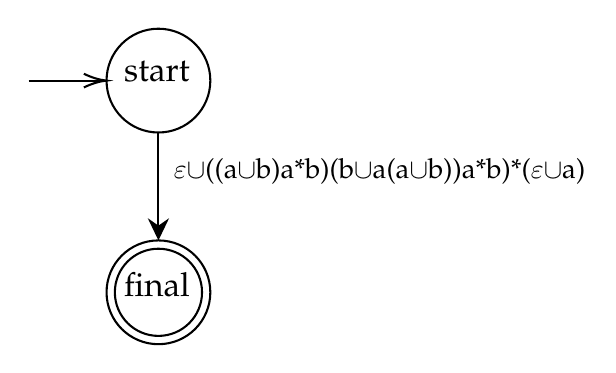
\begin{tikzpicture}[x=0.75pt,y=0.75pt,yscale=-1,xscale=1]
%uncomment if require: \path (0,180); %set diagram left start at 0, and has height of 180

%Shape: Circle [id:dp3675772978743408] 
\draw   (51,34) .. controls (51,20.19) and (62.19,9) .. (76,9) .. controls (89.81,9) and (101,20.19) .. (101,34) .. controls (101,47.81) and (89.81,59) .. (76,59) .. controls (62.19,59) and (51,47.81) .. (51,34) -- cycle ;
%Straight Lines [id:da8787222323554729] 
\draw    (13.5,34) -- (49,34) ;
\draw [shift={(51,34)}, rotate = 180] [color={rgb, 255:red, 0; green, 0; blue, 0 }  ][line width=0.75]    (10.93,-3.29) .. controls (6.95,-1.4) and (3.31,-0.3) .. (0,0) .. controls (3.31,0.3) and (6.95,1.4) .. (10.93,3.29)   ;
%Shape: Circle [id:dp19089431232049026] 
\draw   (51,136) .. controls (51,122.19) and (62.19,111) .. (76,111) .. controls (89.81,111) and (101,122.19) .. (101,136) .. controls (101,149.81) and (89.81,161) .. (76,161) .. controls (62.19,161) and (51,149.81) .. (51,136) -- cycle ;
%Shape: Circle [id:dp11775682029954848] 
\draw   (55,136) .. controls (55,124.4) and (64.4,115) .. (76,115) .. controls (87.6,115) and (97,124.4) .. (97,136) .. controls (97,147.6) and (87.6,157) .. (76,157) .. controls (64.4,157) and (55,147.6) .. (55,136) -- cycle ;
%Straight Lines [id:da8742799689860312] 
\draw    (76,59) -- (76,108) ;
\draw [shift={(76,111)}, rotate = 270] [fill={rgb, 255:red, 0; green, 0; blue, 0 }  ][line width=0.08]  [draw opacity=0] (10.72,-5.15) -- (0,0) -- (10.72,5.15) -- (7.12,0) -- cycle    ;

% Text Node
\draw (58,23) node [anchor=north west][inner sep=0.75pt]  [font=\large] [align=left] {start};
% Text Node
\draw (58,125) node [anchor=north west][inner sep=0.75pt]  [font=\large] [align=left] {final};
% Text Node
\draw (82,70) node [anchor=north west][inner sep=0.75pt]   [align=left] {$\displaystyle \varepsilon \cup $((a$\displaystyle \cup $b)a*b)(b$\displaystyle \cup $a(a$\displaystyle \cup $b))a*b)*($\displaystyle \varepsilon $$\displaystyle \cup $a)};


\end{tikzpicture}

\end{enumerate}

\end{enumerate}

\newpage

\begin{prob}\end{prob}

\begin{enumerate}[label=(\alph*)]

\item
$p \neq 0$ because the only zero-length string in the language is $\varepsilon$, which cannot be pumped. \\
$p = 1$ works, because we can pump the first character in the string, whether it is $0$,
which will be covered by $0^*$, or it is $1$, which is covered by $1^*$. There are no strings in
the language that is $1$ followed by a $0$, so $0^* 1^*$ covers all our cases.

\item
$p \neq 1$ because we can simply choose one character in the $01$, and then we will have either $0^* 1$ or $01^*$, 
neither of which fits $(01)^*$. \\
$p = 2$ works, because we can then pick the first occurence of $01$ and pump that. 

\item
$p \neq 0$ because the only zero-length string in the language is $\varepsilon$, which cannot be pumped. \\
$p = 1$ works, because the set of words of at least length is $\varnothing$, to which the statment becomes
vacuously true.  

\item
$p \neq 2$ because $00$ cannot be pumped. The restriction is that there are exactly two zeroes, which pumping
will break if we pick either $0$. \\
$p = 3$ works, because we can pump the $1$, wherever it appears.

\item
$p \neq 3$ because in $100$, $10$ cannot be pumped down, only up. \\
$p = 4$ works, because the first $w \in A$ we can use is $10100$, in which we pick the second $10$. This
can be pumped up or down, since $(10)*$ will fit under $(11*0)*$. 

\item
$p \neq 4$ because $1011$ is of length 4, and anything we pump will not be in the set. \\
$p = 5$ works, because there are not strings of at least length 5, which leaves us $\varnothing$ to pump,
which is vacuously true.

\item
$p \neq 0$ because the only zero-length string in the language is $\varepsilon$, which cannot be pumped. \\
$p = 1$ works, because we can simply pump the first character. $\Sigma^*$ is a language that includes
all substrings with $1$ and $0$.

\end{enumerate}

\begin{prob}\end{prob}

\noindent $p \neq 3$ because a counter example is $000$, where no matter what is pumped, there will eventually be $0000$ as a substring. \\
$p = 4$ works, because we can pump the first four letters in $w$. We know that the word does not contain $0000$ nor $1111$, and 
and repeating the same word cannot produce $0000$ or $1111$, because there is no 4-letter word that both begins and ends with 
$00$ and is not $0000$. Same is true for $1111$.


\newpage

\begin{prob}\end{prob}

\begin{enumerate}[label=(\alph*)]

\item
Assume that $L = \{ w w^R | w \in \{a, b\}^*\}$ is regular. Then, there must be some pumping length 
$p$. Consider $w = a^p b^p b^p a^p$. We have $w \in L$ and $|w| \geq p$. If we let $y = a^p$, 
and $x = \varepsilon$ and $z = b^p b^p a^p$, we can pump $y$ up or down, which will break the symmetry
of $a$'s to the left and right of the center. This broken symmetry creates a contradiction, because 
$L = \{ w w^R | w \in \{a, b\}^*\}$ is symmetric words only. Thus, $L$ cannot be regular.

\item
Assume that $L = \{ w \bar{w} | w \in \{a, b\}^*\}$ is regular. Then, there must be some pumping length
$p$. Consider $w = a^p b^p$. We have $w \in L$ and $|w| \geq p$. If we let $y = a^p$, $x = \varepsilon$,
and $z = b^p$, we can pump $y$ up or down, breaking the equal parity of $a$ and $b$s. This
generates a word that is not in $L$, which creates a contradiction. Thus, $L$ cannot be regular.

\end{enumerate} 

\begin{prob}\end{prob}

Assume that $L = \{ a^t | t \text{ is a prime number}\}$ is regular. Then, there must be some pumping length
$p$. Consider $w = a^p a^{t - p}$ where $t$ is a prime number and $t \geq p$. Then, $w \in L$ and 
$|w| \geq p$. If we let $y = a^p a^{t - p}$, $x = \varepsilon$ and $z = \varepsilon$. If we then pump $y$,
to some whole number $n$, we would get $w = a^{np} a^{n(t - p)}$, which can be simplified to $w = a^{nt}$. 
This $w \notin L$, because $nt$ is by definition not prime. Therefore, we have a contradiction. $L$ cannot be regular.

\end{document}
